\section{3D Results}
In previous sections, we showed that changing the streaming order can significantly reduce error at given position
in the stream. For example, adaptive RMSE optimized stream outperforms any fixed ordering stream, such as by level,
by bitplane, or by wavelet norm. Moreover, we performed an extensive study on various 2D datasets which shows that
data-dependent stream order offers best results.

However, all experiments were done on mostly on 2D slices of 3D data, since those can be inspected manually in our
tool (\pavol{REF}) and the stream and error computation takes orders of magnitude less time. To validate the results
apply to 3D data, we run the same experiments on the full 3D data sets. Since, the data sets are much larger, we had
to for practical reasons increase the group size from $4^2$ to $16^3$.

We start with reproducing the experiment comparing streaming the data \emph{by level}, \emph{by bit plane},
and \emph{by wavelet norm} (\Cref{fig:motivation-3d-rmse}). In 2D experiments, all data set exhibited the by level
being the worst order, then by bit plane, and the best was by wavelet norm (REF). The 3D results are different as
the by level an by bit plane orders cross. \pavol{WHY?, especially boiler does not have almost any empty space}

\begin{figure}
  \centering
	\subcaptionbox{Boiler}
  {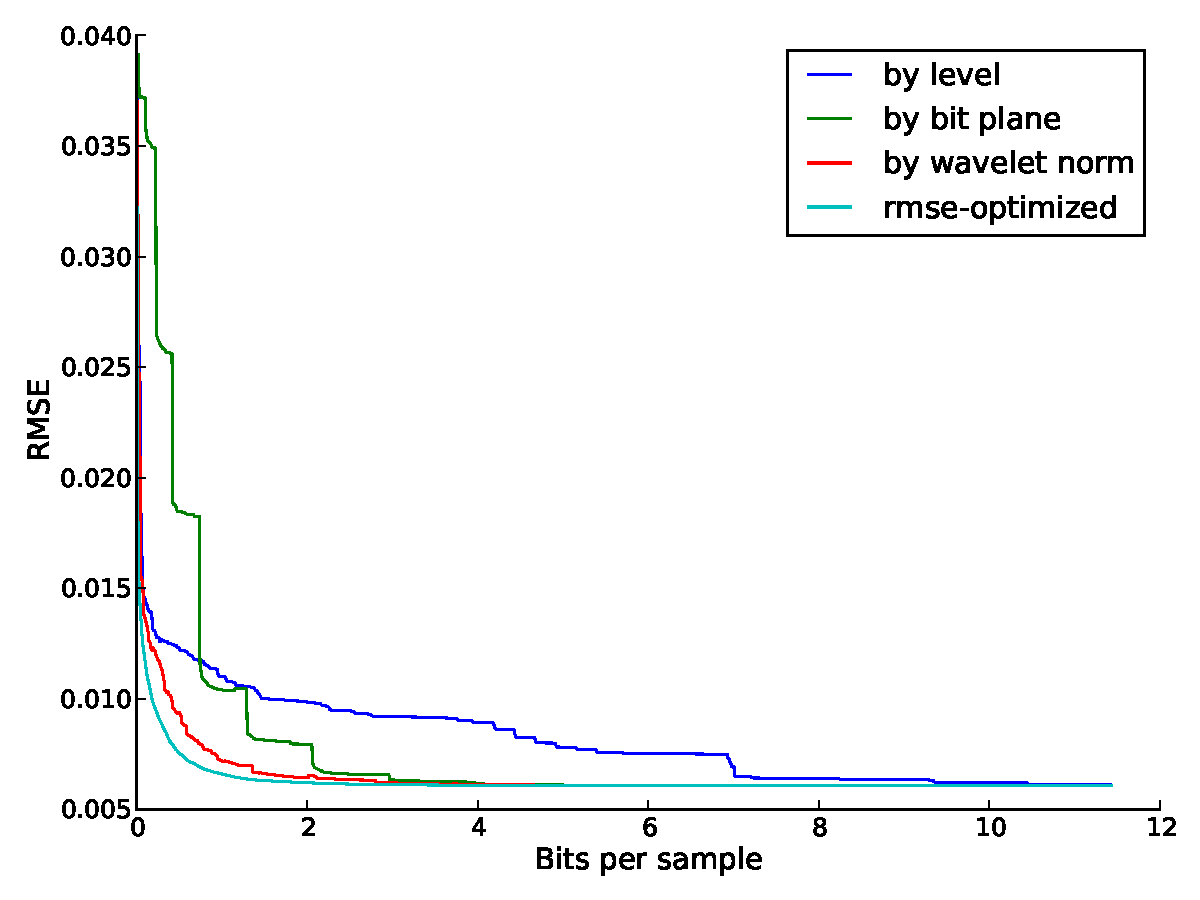
\includegraphics[width=0.48\linewidth]{img/motivation-3d/rmse-boiler.pdf}}
	\subcaptionbox{Diffusivity}
 	{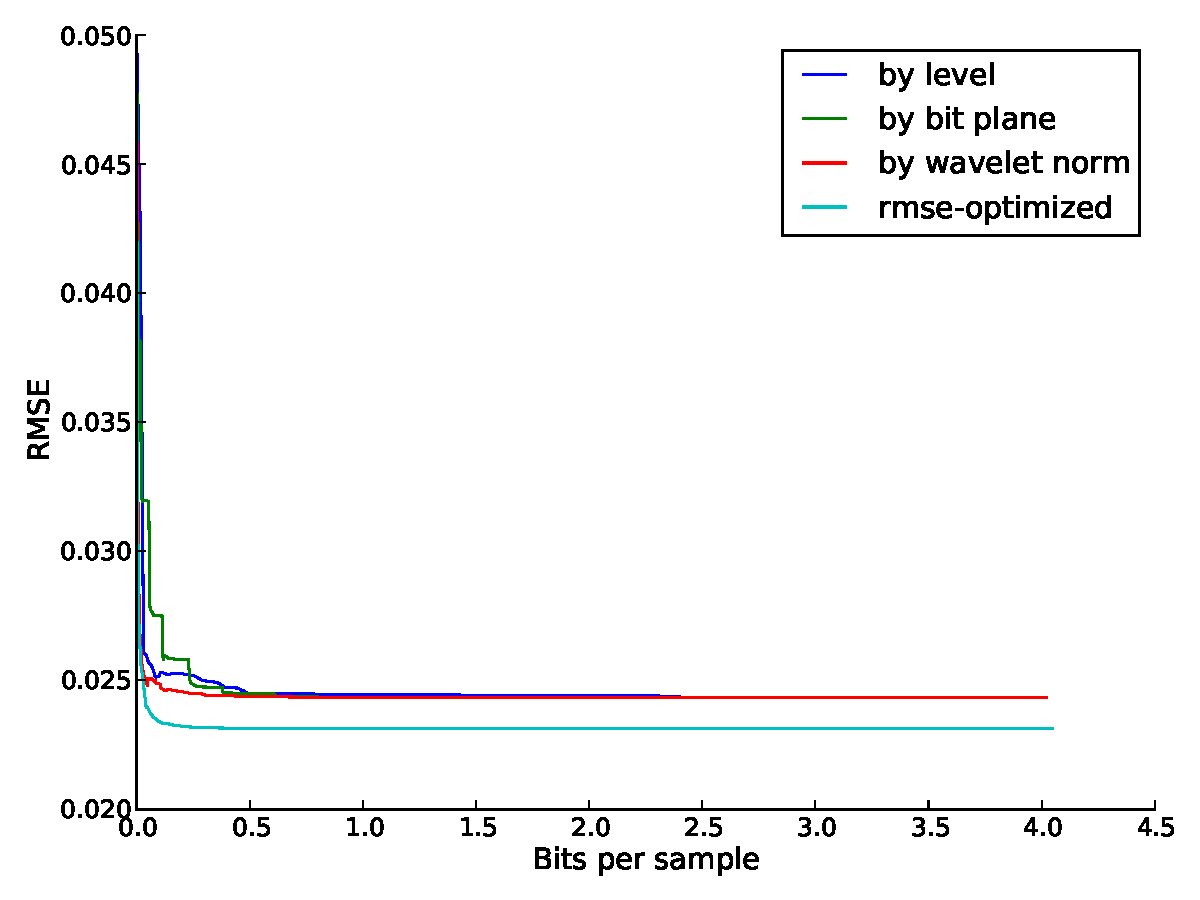
\includegraphics[width=0.48\linewidth]{img/motivation-3d/rmse-diffusivity.pdf}}
	\subcaptionbox{Turbulence}
 	{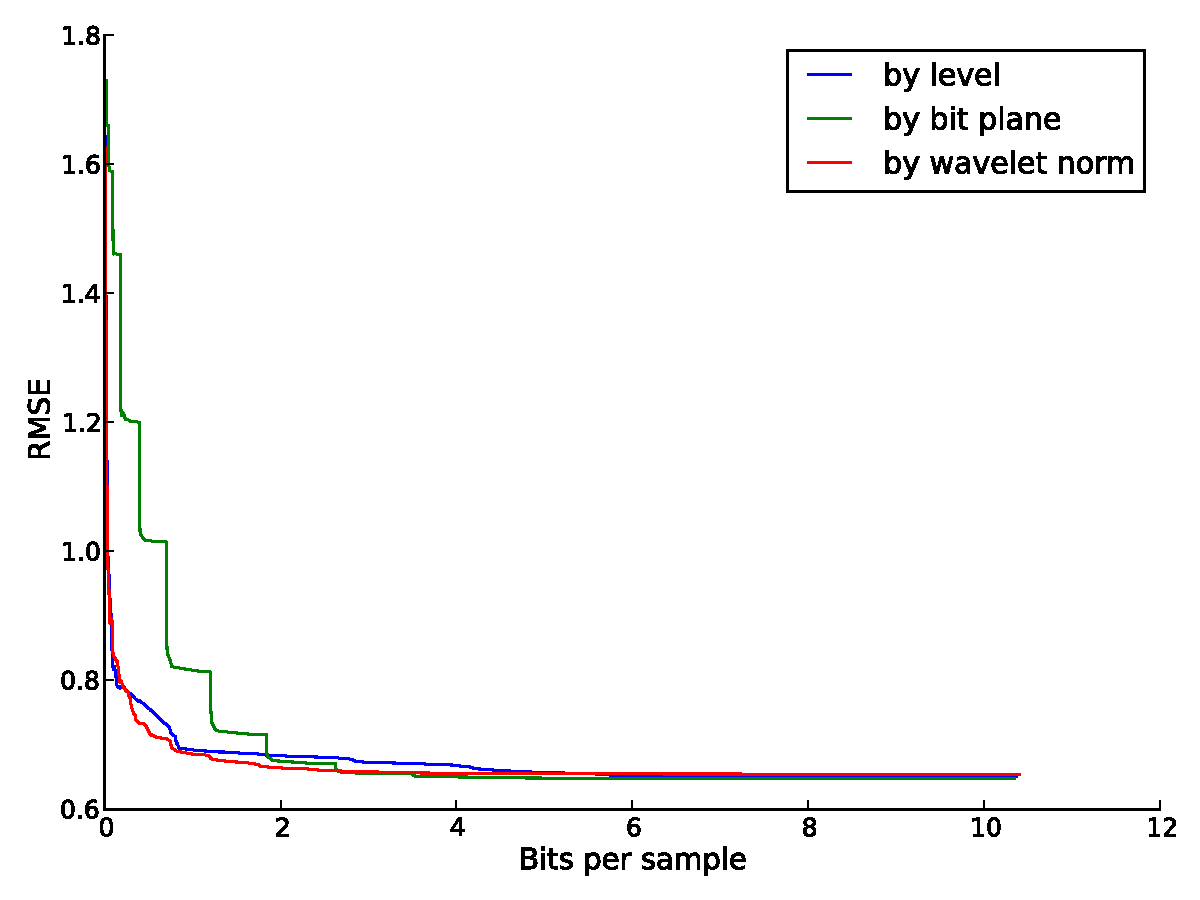
\includegraphics[width=0.48\linewidth]{img/motivation-3d/rmse-turbulence.pdf}}
	\subcaptionbox{Velocity-z}
 	{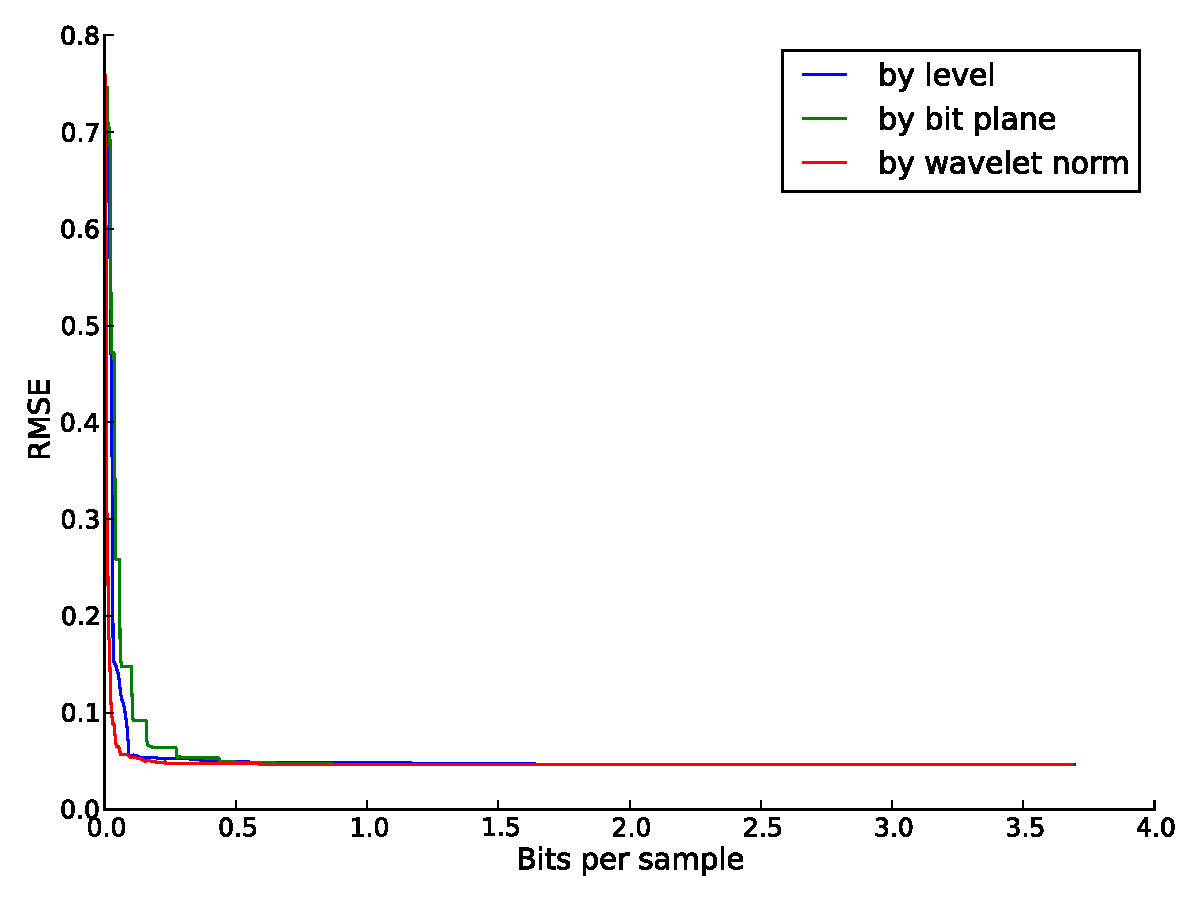
\includegraphics[width=0.48\linewidth]{img/motivation-3d/rmse-velocityz.pdf}}
 	\caption{Root-mean-square error of reconstructed functions using the three data-agnostic streams
 	defined in Section \ref{sec:motivation}. Lower is better. The streams are truncated to highlight
 	the differences, without omitting important information. \emph{by wavelet norm} performs best,
 	followed closely by \emph{by bit plane}. We left out \emph{euler} (2D) and \emph{plasma} (buggy) datasets.}
 	\label{fig:motivation-3d-rmse}
\end{figure}


